% !TEX root = ../Thesis.tex
%%
%%  Hochschule für Technik und Wirtschaft Berlin --  Abschlussarbeit
%%
%% Kapitel 3 - Konzept / Architektur
%%
%%

%\chapter{Konzeption} \label{Konzept}

\section{Test}

Für die Umsetzung einer Wasseroberflächenüberwachung wurden in dieser Arbeit viele Entscheidungen gefällt, die sich konkret mit den limitierenden Faktoren auseinander setzen. Diese sind insbesondere: 

Kritische Infrastruktur
Die Berliner Wasserbetriebe haben als Versorger des Landes Berlin und Umgebung eine große Verantwortung und Sorgfaltspflicht gegenüber den Konsumenten und Nutzern. Auch die Abwasserentsorgung unterliegt dementsprechend strengen Richtlinien, die Auswirkungen auf Arbeitsprozesse genommen haben.
So ist die Wahl eines Air-Gaps in der Hardware als höchste Sicherheitsstufe unmittelbar darauf zurückzuführen. Diese simple Entscheidung hat bereits gravierende Auswirkungen auf unterschiedlichste Lösungsansätze genommen wie das Betreiben eines Zweitrechners zum Überspielen der Daten, die Wahl des Neuronalen Netzes in seinem Aufbau und die Datenerfassung selbst.

\textbf{Ergänzen}: kurzes Sicherheits-/Threat-Model (welche Angreifer/Fehlerszenarien, welche Daten sind sensibel), sowie konkrete Konsequenzen für Betrieb/Updates: wie gelangen Trainingsdaten/Modelle/Logs über den Air-Gap (Medium, Prozess, Verantwortlichkeiten)?

Da das Bilderfassungssystem im Außeneinsatz positioniert ist, ergeben sich umfassende Anforderungen in Anbetracht der physischen Anbindung an die Peripherie, dem Umgang mit Witterungsbedingungen als auch Zuverlässigkeit und Wartungsminimierung. 

Zeit ist immer ein limitierender Faktor, wenn es um die Einarbeitung in ein fachfremdes Thema geht, in dem die Betrachtung von Umständen notwendig ist, mit denen man sich weder selbst noch jemand anderes in dem Bereich bereits auseinandergesetzt hat. Entsprechend sind Design-Entscheidungen dann auch relevant, wenn es um die Planung und Skalierung von Ressourcen geht. So ist bei der Beschaffung von Materialien immer auch mit der Umgebung zu rechnen und der Umfang entsprechend klein zu halten. 

\section{Entwurf des eigenen Lösungskonzepts}


    
\begin{figure}[h]
    \centering
    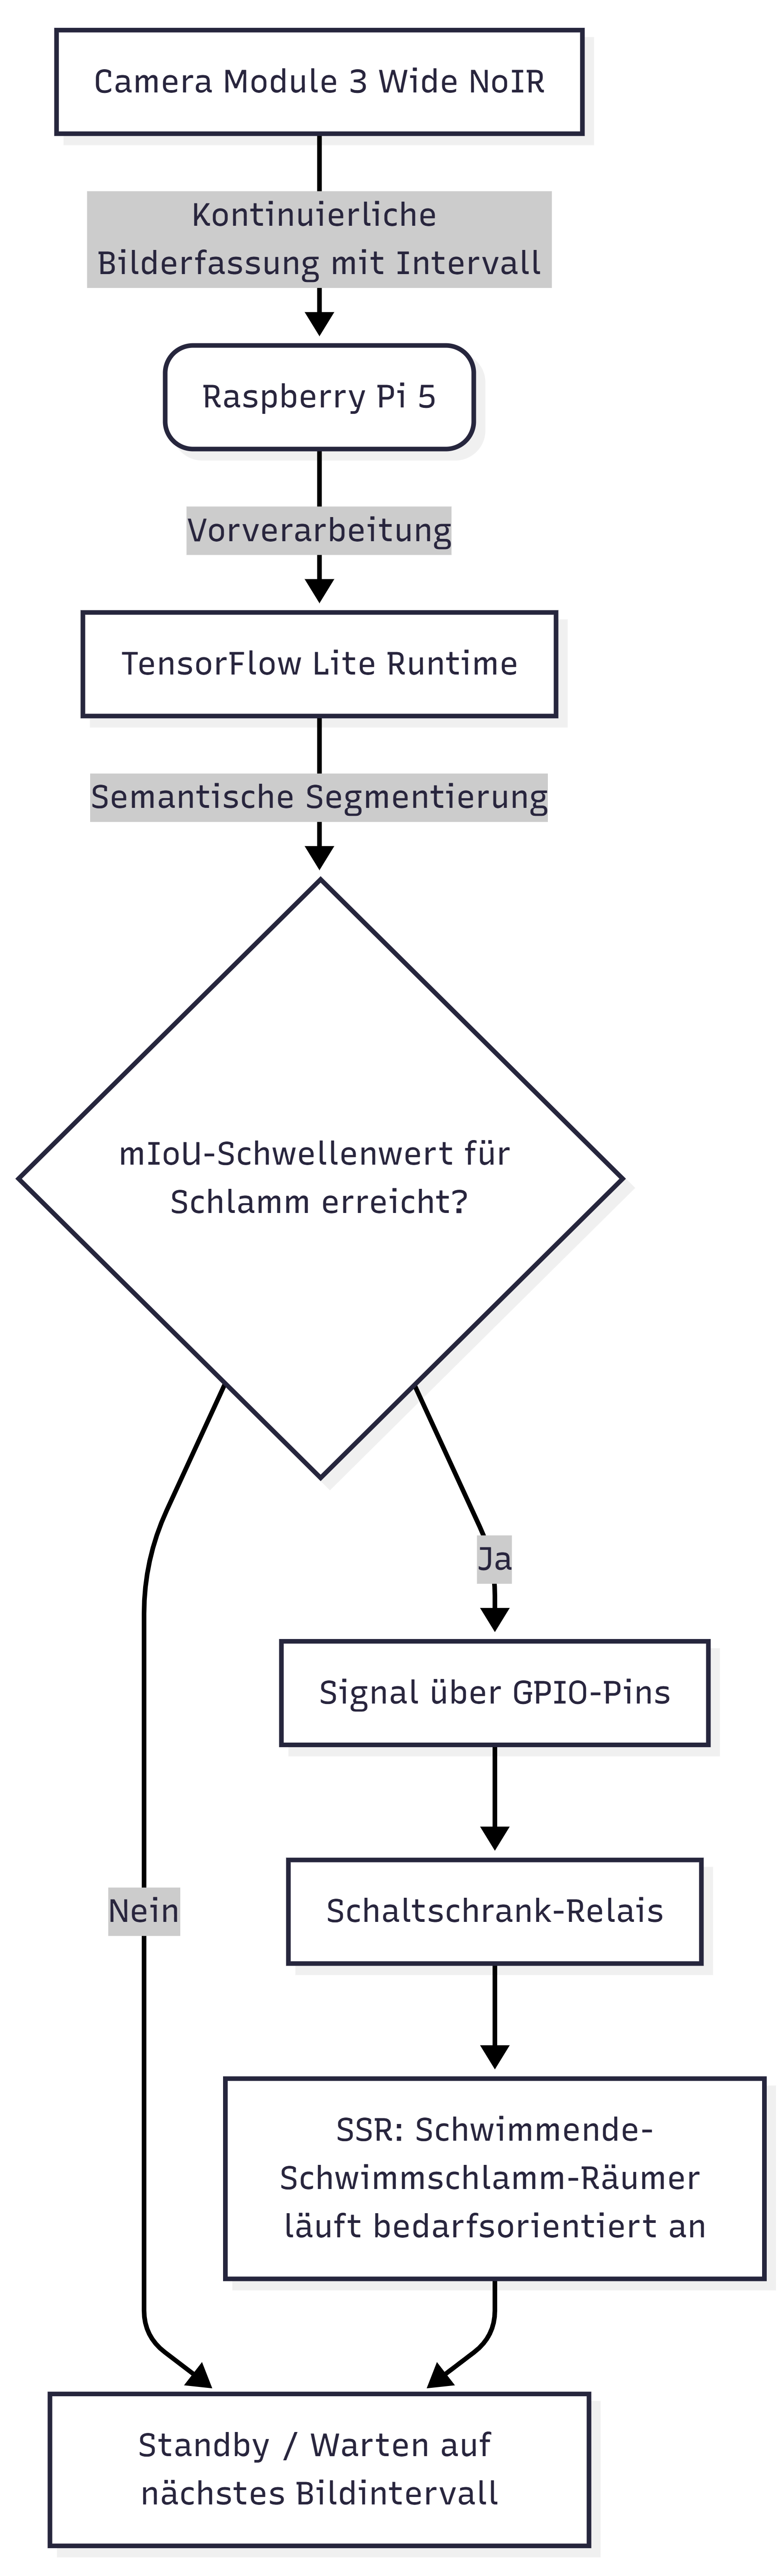
\includegraphics[width=0.4\linewidth]{pictures/Bildverarbeitung.png}
    \caption{Visualisierung der Bildverarbeitungspipeline}
    \label{fig:Bildpipeline}
\end{figure}
    
    




\pagebreak

\textbf{Ausformulieren}: Konzept als durchgängiger Daten-/Steuerungsfluss (Kamera $\rightarrow$ Preprocessing $\rightarrow$ Modell $\rightarrow$ Entscheidung $\rightarrow$ Aktorik). Danach die Entscheidung begründen (Kriterien, Alternativen, warum verworfen). Vorteil/Nachteil-Liste in argumentativen Text überführen und mit Anforderungen verknüpfen.

    


\begin{table}[]
\begin{tabular}{|l|l|l|}
\hline
\textit{\textbf{Komponente}} & \textit{\textbf{Vorteile}} & \textit{\textbf{Nachteile}} \\ \hline
\textbf{Raspberry Pi 5}      & Preiswert                  & Schlechte Skalierbarkeit    \\ \hline
                             & Anpass- und erweiterbar    & Kein Industriestandard      \\ \hline
                             & Perfomant                  & Hoher Wartungsaufwand       \\ \hline
                             & Open Source                & Lokal beschränkt            \\ \hline
                             & Anbindungsmöglichkeit      & Komplexer Systemaufbau      \\ \hline
                             & Lokal trainierbar          &                             \\ \hline
\textbf{Edge-AI Cam}         & Hohe Skalierbarkeit        & Teuer                       \\ \hline
                             & Industriestandard          & Geschlossenes System        \\ \hline
                             & Niedriger Wartungsaufwand  & Externe Ressourcen          \\ \hline
                             & Hoher Stromverbrauch       & Hoher Planungsaufwand       \\ \hline
                             & Netzwerkweit angebunden    &                             \\ \hline
                             & Simple Benutzeroberfläche  &                             \\ \hline
\end{tabular}
\end{table}

\begin{itemize}
\item Darstellung des eigenen Ansatzes, ggf. Abgrenzung von anderen Arbeiten
\item Vorteile
\begin{itemize}
    \item Preiswerter Einplatinencomputer
    \item Gute Anpassungs- und Erweiterungsmöglichkeiten
    \item Hohe Performance
    \item Open Source
    \item Unkomplizierte Anbindung
    \item Lokal trainierbar
\end{itemize}
\item Nachteile
\begin{itemize}
    \item Schlechte Skalierbarkeit
    \item Kein Industriestandard
    \item Hoher Wartungsaufwand
    \item Hoher Stromverbrauch ?
    \item Lokal beschränkt
    \item Geringe Systemeinsicht
\end{itemize}

\end{itemize}
\section{Auswahl/Entwurf der Hardware}

\begin{table}[]
\begin{tabular}{|l|l|l|l|l|l|} \hline
\textbf{Komponente}          & \textbf{Aufgabe}                                       & \textbf{Spezifikation}             & \textbf{CPU}                     & \textbf{RAM} \\ \hline 
ThinkPad T14 & Internet & 256 GB SSD                            & Intel i5-1135G7         & 32 GB 2700 MHz   \\ \hline
Pro Rugged 14  & Coding                          & 2 TB SSD                              & Intel Ultra 5 125U x 12 & 32 GB 5600 MHz \\ \hline
Pi 5      & Verbindung                           & 64 GB SD-Karte                        & Broadcom BCM2712        & 8 GB 4267 MHz \\ \hline
Camera Module 3     & Peripherie                                    & Wide-NoIR & -                       &   - \\ \hline
\end{tabular}
\end{table}


Für die praktische Umsetzung des Edge-Computing-Systems zur Wasseroberflächenüberwachung wird eine dedizierte Hardware-Architektur benötigt, die den strengen Vorgaben der Air-Gap-Umgebung sowie den harschen Bedingungen vor Ort am Nachklärbecken gerecht wird. Die Infrastruktur teilt sich hierbei in drei primäre Rechenleistungen und eine optische Erfassungskomponente auf:  Als primäres Arbeitsgerät für den administrativen und netzwerkgebundenen Teil der Arbeit kommt ein Lenovo ThinkPad T14 zum Einsatz. Aufgrund der Sicherheitsrichtlinien der Berliner Wasserbetriebe dient dieses Endgerät ausschließlich als Schnittstelle zur Außenwelt, um die notwendige Internetanbindung für die globale Informationsbeschaffung zu gewährleisten. Darüber hinaus wird dieses System für die cloudbasierte oder lokale Textdokumentation der Ausarbeitungen genutzt.  Für die rechenintensiven Prozesse des Projekts wird ein robustes Notebook vom Typ Dell Latitude Pro Rugged herangezogen. Dieses System agiert innerhalb der Air-Gap-Umgebung komplett offline. Seine Hauptaufgaben liegen im lokalen Training des Neuronalen Netzes, der direkten Kommunikation und Konfiguration des Edge-Geräts via Kabelverbindung sowie der anschließenden mathematischen und statistischen Auswertung der Testergebnisse.  Die eigentliche Ausführung des KI-Modells direkt am Prozess (Edge-Computing) übernimmt ein Raspberry Pi 5. Dieser zeichnet sich durch eine hohe Recheneffizienz bei geringer Leistungsaufnahme aus und ist für die kontinuierliche Datenerfassung der Bildströme sowie die anschließende Peripheriesteuerung des Schwimmenschlamm-Räumers (SSR) verantwortlich.  Die optische Datenerfassung erfolgt über das Raspberry Pi Camera Module 3 Wide NoIR. Die Wahl fiel explizit auf die NoIR-Variante (No Infrared), um über externe Infrarotscheinwerfer eine lückenlose Nachtsicht und Ausleuchtung der Wasseroberfläche zu realisieren. Das Weitwinkelobjektiv (Wide) garantiert hierbei einen maximalen Erfassungswinkel, um die relevanten Bereiche des Nachklärbeckens optimal abzubilden. Zur Reduktion von störenden Lichtreflexionen und Spiegelungen auf der Wasseroberfläche wird die Optik zudem durch einen dedizierten Polarisationsfilter ergänzt.

\section{Auswahl/Entwurf der Software}
Parallel zur Hardware-Struktur erfordert das System eine harmonisierte Software- und Betriebssystemlandschaft, die den Offline-Betrieb und den Entwicklungsprozess lückenlos unterstützt.


\subsection{Betriebssysteme}

Auf den jeweiligen Hardwarekomponenten kommen drei differenzierte Betriebssysteme zum Einsatz:
Das \textit{Lenovo ThinkPad T14} wird unter \textbf{Windows 11 Enterprise} betrieben, was den Unternehmensstandards entspricht und eine sichere Verbindung zu den internen und externen Netzwerken erlaubt.
Auf dem \textit{Dell Pro Rugged} wird die Linux-Distribution \textbf{Linux Mint} mit der \textbf{Cinnamon-Benutzeroberfläche} eingesetzt. Diese Wahl begründet sich in der hohen Stabilität, der exzellenten Unterstützung für Entwicklerwerkzeuge und der Ressourceneffizienz im Offline-Betrieb.
Als Betriebssystem für die Edge-Plattform (Raspberry Pi 5) wird das offizielle, Debian-basierte \textbf{Raspberry Pi OS} verwendet, da dieses eine native Treiberunterstützung für das genutzte Kameramodul und die GPIO-Schnittstellen bietet.


\subsection{Softwarekomponenten nach System}

    


\begin{enumerate}
    \item \textbf{Lenovo Thinkpad T14:}
    Für die wissenschaftliche Ausarbeitung der Arbeit wird das kollaborative Online-LaTeX-System \textbf{Overleaf} genutzt. Die Erstellung der Ground-Truth-Daten und die manuelle Annotation der Bilddatensätze erfolgt über das webbasierte Tool \textbf{CVAT} (Computer Vision Annotation Tool).
    \item \textbf{Dell Pro Rugged:}
    Die lokale Softwareentwicklung und das Skript-Debugging werden in der Entwicklungsumgebung \textbf{Visual Studio Code} durchgeführt. Zur softwareseitigen Umsetzung der KI-Infrastruktur bildet die Python-Distribution \textbf{Anaconda} das Fundament, welche das Paket- und Environment-Management im Offline-Modus erleichtert. Das Training und die Evaluierung des semantischen Segmentierungsmodells basieren auf den Deep-Learning-Frameworks \textbf{Tensorflow} und \textbf{Keras}, während \textbf{Tensorboard} zur visuellen Analyse und Überwachung der Trainingsmetriken (wie Loss und IoU) eingesetzt wird. Bildverarbeitungsoperationen sowie mathematische Matrixoperationen werden über die Bibliotheken \textbf{OpenCV} und \textbf{NumPy} händisch implementiert.
    \item \textbf{Raspberry Pi 5:}
    Um den KI-Inferenzprozess auf dem Edge-System so performant und ressourcenschonend wie möglich zu gestalten, wird auf dem Kleinstcomputer auf die vollständige Tensorflow-Bibliothek verzichtet. Stattdessen kommt exklusiv die schlanke \textbf{TensorFlow Lite Runtime} (\textit{TFlite Runtime}) zum Einsatz, welche für die ressourceneffiziente Echtzeit-Segmentierung des Bildmaterials optimiert ist.
\end{enumerate}



\begin{lstlisting}[caption=Code zur Umwandlung von .mp4 zu .png]
import cv2
import os

video_path = "/home/oem/Desktop/BIldmaterial/IMG_0002.MOV"
output_dir = "extracted_images"
interval_seconds = 1  

if not os.path.exists(output_dir):
    os.makedirs(output_dir)

cap = cv2.VideoCapture(video_path)
fps = cap.get(cv2.CAP_PROP_FPS)
interval_frames = int(fps * interval_seconds)

count = 0
image_id = 0

while cap.isOpened():
    ret, frame = cap.read()
    if not ret: break
    
    if count % interval_frames == 0:
        cv2.imwrite(f"{output_dir}/img_{image_id:04d}.png", frame)
        image_id += 1
    count += 1

cap.release()
print(  )
print(f"Fertig! {image_id} Bilder exportiert.")
\end{lstlisting}

\begin{lstlisting}[caption=Code zur Maskengenerierung in]
    import cv2
import numpy as np
import os
from os import path
from os import listdir
from cv2 import cvtColor
from cv2 import imread

input_folder = '/home/oem/Desktop/CVAT/extracted_images'
output_folder = '/home/oem/Desktop/CVAT/masked_images/SegmentationClass'
num_classes = 2
register_file = '/home/oem/Desktop/CVAT/masked_images/Segmentation/default.txt'

os.makedirs(output_folder, exist_ok=True)

os.remove(register_file)

def auto_annotate(image_path):
    img = cv2.imread(image_path, flags=cv2.IMREAD_COLOR)
    hsv = cv2.cvtColor(img, cv2.COLOR_BGR2HSV)

    lower_blue = np.array([20, 20, 20])
    upper_blue = np.array([255, 255, 255])

    contra_upper_blue = np.array([0, 0, 0])

    mask3 = cv2.inRange(hsv, lower_blue, upper_blue)
    mask4 = cv2.inRange(hsv, contra_upper_blue, lower_blue)

    #Rauschen filter - optional
    kernel = np.ones((5,5), np.uint8)
    mask3 = cv2.morphologyEx(mask3, cv2.MORPH_OPEN, kernel)

    #Hintergrund-Klasse
    combined_mask = np.zeros(mask3.shape, dtype=np.uint8)

    combined_mask[mask3 > 0] = 1 
    return combined_mask

    base_name = os.path.basename(image_path).split('.')[0]

    #Konvertierung zu numerischen Arrays
    cv2.imwrite(os.path.join(output_folder, f"{base_name}_mud.png"), mud_mask.astype(np.uint))
    cv2.imwrite(os.path.join(output_folder, f"{base_name}_water.png"), water_mask.astype(np.uint))

    return mud_mask, water_mask

for images in os.listdir(input_folder):
    mask = auto_annotate(os.path.join(input_folder, images))
    out_name = (images)
    
    name_wo_extension = os.path.splitext(images)[0]

    with open(register_file, "a") as f:
        f.write(name_wo_extension + "\n") 
        
        cv2.imwrite(os.path.join(output_folder, out_name), mask)
        
with open(register_file) as lines:
    names = list(lines)
names.sort()
print(names)


\end{lstlisting}

%\subsection{Entwurf von Lösungsmodulen}




